\subsection{Numerical Solutions for Burgers' Equation without Viscosity}
	
	To finish the section, we will study the problem (\ref{IVP_Burgers}) without viscosity, that is, when $\alpha = 0$. So the problem is the following
	\begin{align}
	\label{IVP_Inviscid}
		\left \lbrace \begin{array}{ll}
			\frac{\partial u}{\partial t} + \frac{1}{2} (u^2)_x = 0, \hspace{2mm} 0 < t \leq T, \hspace{2mm} x \in \mathcal{D} \\
			\\
			u(x, 0) = u_0(x), \hspace{2mm} x \in \mathcal{D}
		\end{array}  \right .
	\end{align}

	This problem, which seems much simpler, turns out to be very interesting, because it presents relevant characteristics regarding the physical interpretation of the problem in general, that is, the case with non-zero viscosity. \\
	
	The previous equation interprets the conservation of energy and is considered as a non-linear conservation law. We can understand this if we consider the function $ u $ as the speed of a fluid that conserves its energy with a flow density given by $f(u) = \frac{u^2} {2}$. \\
	
	The above can be shown considering that $u \in H^1_p [\mathcal{D}]$, and multiplying by $u$ and integrating both sides of the equation on the domain $\mathcal{D}$ to prove that $\| u \|$ does not change over time, that is,
	\begin{align*}
		\frac{1}{2} \frac{d}{dt} \displaystyle \int_{0}^{2 \pi} u^2(x, t) dx = - \int_{0}^{2 \pi} u^2(x, t) \frac{\partial u(x, t)}{\partial x} dx = - \frac{1}{3} u^3(x, t) \Big|^{2 \pi}_{0}.
	\end{align*}
	and because $u$ is periodic, we have to
	\begin{align*}
		\frac{1}{2} \frac{d}{dt} \| u(x, t) \|^2 = 0.
	\end{align*}
	This means that the energy is conserved with the same initial energy since we must bear in mind that this represents the kinetic energy of a fluid that travels with a velocity given by $u_0$. \\
		
	In any problem, these characteristics are of utmost importance, this is because we must consider the behavior of the solutions when they must be approached with some numerical method. In the literature, when a solution remains bounded in time, the problem is said to be well defined. In the analysis context, this assures us the existence of a continuously differentiable solution $u$, and that besides being unique, it is possible to approximate it. \\
	
	However, approximating the solutions to this problem using spectral methods can be more complicated if its characteristics are not well understood. Next, we will see that under a certain condition it is possible to find a single analytical solution and that otherwise, it may lose its uniqueness when developing discontinuities. \\
			
	First, let's define the curves $x = x(t)$ that start at a point $x_0 \in \mathbb{R}$, and satisfy the following problem
	\begin{align*}
		\left \lbrace \begin{array}{ll}
			x' (t) = u(x(t), t), \hspace{2mm} t > 0, \\
			\\
			x(0) = x_0.
		\end{array} \right .  
	\end{align*}
	
	The solutions for each $x_0$ are known as characteristic curves, which pass through the solution $u = u (x (t), t)$. It is well known in the theory of differential equations that when $u(x, t)$ is locally Lipschitz in the variable $x$, and continues in the variable $t$, the above equation admits a single solution $x(t)$ for each $x_0 \in \mathbb{R}$. So, assuming the above we have that for a solution $ x (t) $ corresponding to a fixed $x_0 \in \mathbb{R}$, it satisfies the following
	\begin{align*}
		\frac{d}{dt} [u(x(t), t)] &= x' (t) u_x (x(t), t) + u_t (x(t), t) \\
		&= u(x(t), t) u_x (x(t), t) - u(x(t), t) u_x (x(t), t) = 0
	\end{align*}
	which tells us that the function $u(x (t), t)$ is independent of the variable $t$, remaining constant along the characteristic curve. Therefore, we have to
	\begin{align*}
		u(x(t), t) = u (x(0), 0) = u_0 (x_0)
	\end{align*}
	
	Furthermore, we have that the solution $ x (t) $ will be given by the following curve
	\begin{align*}
		x(t) = x_0 + u_0 (x_0) t, \hspace{2mm} t > 0.
	\end{align*}
	which allows us to write the solution $ u(x, t)$ as follows
	\begin{align}
	\label{Exact_Inviscid}	
		u(x, t) = u_0(x_0), \hspace{2mm} x_0 = x - u_0(x_0) t
	\end{align}
	
	Note that the Lipschitz condition is necessary for the uniqueness of the above solution, since, conversely, if we set two different starting points $x_0, x_1$ such that $x_0 <x_1$, then its curves characteristics intersect for some $t$, that is,
	\begin{align*}
		x_0 + u_0(x_0) t = x_1 + u_0 (x_1) t,
	\end{align*}
	and using the mean value theorem we have that for some $c \in (x_0, x_1)$ the time $t$ is given by
	\begin{align*}
		t = \frac{x_1 - x_0}{u_0 (x_0) - u_0 (x_1)} = - \frac{1}{u'_0(c)},
	\end{align*}
	
	The above tells us that when these two curves intersect, the solution $u (x, t)$ cannot be continuous in the time $ t $ given by the previous equation. This is because $u_0 (x_0) \neq u_0 (x_1)$, and since the solution is constant over time we would have that $u (x, t) = u_0 (x_0) = u_0 (x_1)$, which is impossible. \\
		
	Therefore, the time $t$ for which two curves intersect represents a discontinuity, and that can be calculated by
	\begin{align}
	\label{shock_time}	
			Tc = \min_{x \in \mathbb{R}} \left[  \frac{-1}{u'_0 (x)} \right]
	\end{align}
	and we can observe that the continuity of the solution $u$ is assured if $T_c < 0$, which depends only on the initial condition $u_0$. \\
	
	This type of information allows us to know the criteria that must be considered when implementing numerical methods, but also the physical interpretation of the problem can be useful. For example, the solution to this problem can be considered to simulate the evolution of the profile of a sea wave that deforms as it approaches the coast until it breaks. But when this occurs, the deformation of the wave stops precisely at the time $T_c$. \\
	
	We must consider that the problem without viscosity supposes that the fluid behaves in an ideal or perfect way, traveling as if they were separate sheets without rubbing. But in real life, fluids always have a certain degree of viscosity, that is, the fluid sheets can rub and cause energy dissipation, and for these cases, we could consider the problem with sufficiently small values ​​of $\alpha$. So a question that naturally arises is what the behavior of the solutions looks like when $\alpha$ approaches zero. \\
	
	In chapter \ref{Introduction} we obtained the solution of the problem (\ref{IVP_Burgers}), which is given by (\ref{Exact_Solution}), and from this equation we can see that the solutions are infinitely differentiable for any value of $\alpha> 0$. Instinctively, we can notice that the solution approaches the solution of the equation without viscosity when $\alpha$ approaches zero. In fact, the solution obtained as a limit when $\alpha$ approaches zero is known as the entropy solution, which has been studied in \cite{Tadmor1989}, \cite{Maday1989} and in \cite{Kruzkov1970} has been proved that this solution is unique. \\
	
	In order to illustrate what we have previously discussed, we will consider the problem (\ref{IVP_Inviscid}) with the following initial condition function
	\begin{align}
	\label{IC_Inviscid}	
		u_0 (x) = e^{-0.005x^2}, \hspace{3mm} x \in \mathcal{D}
	\end{align}
	where $\mathcal{D} = [x_L, x_R]$, and considering the interval $I = [0, T_c]$ for a value of $T_c$ given by (\ref{shock_time}). \\
	
	In the following simulations, we will use the Fourier-Galerkin method given in (\ref{Galerkin_Euler}) to obtain approximations with different values of $\alpha$, and we will see how they approximate the exact solution of the problem (\ref{IC_Inviscid} ) which was given in (\ref {Exact_Inviscid}).
	
	\newpage
	\begin{figure}[H]
		\centering
		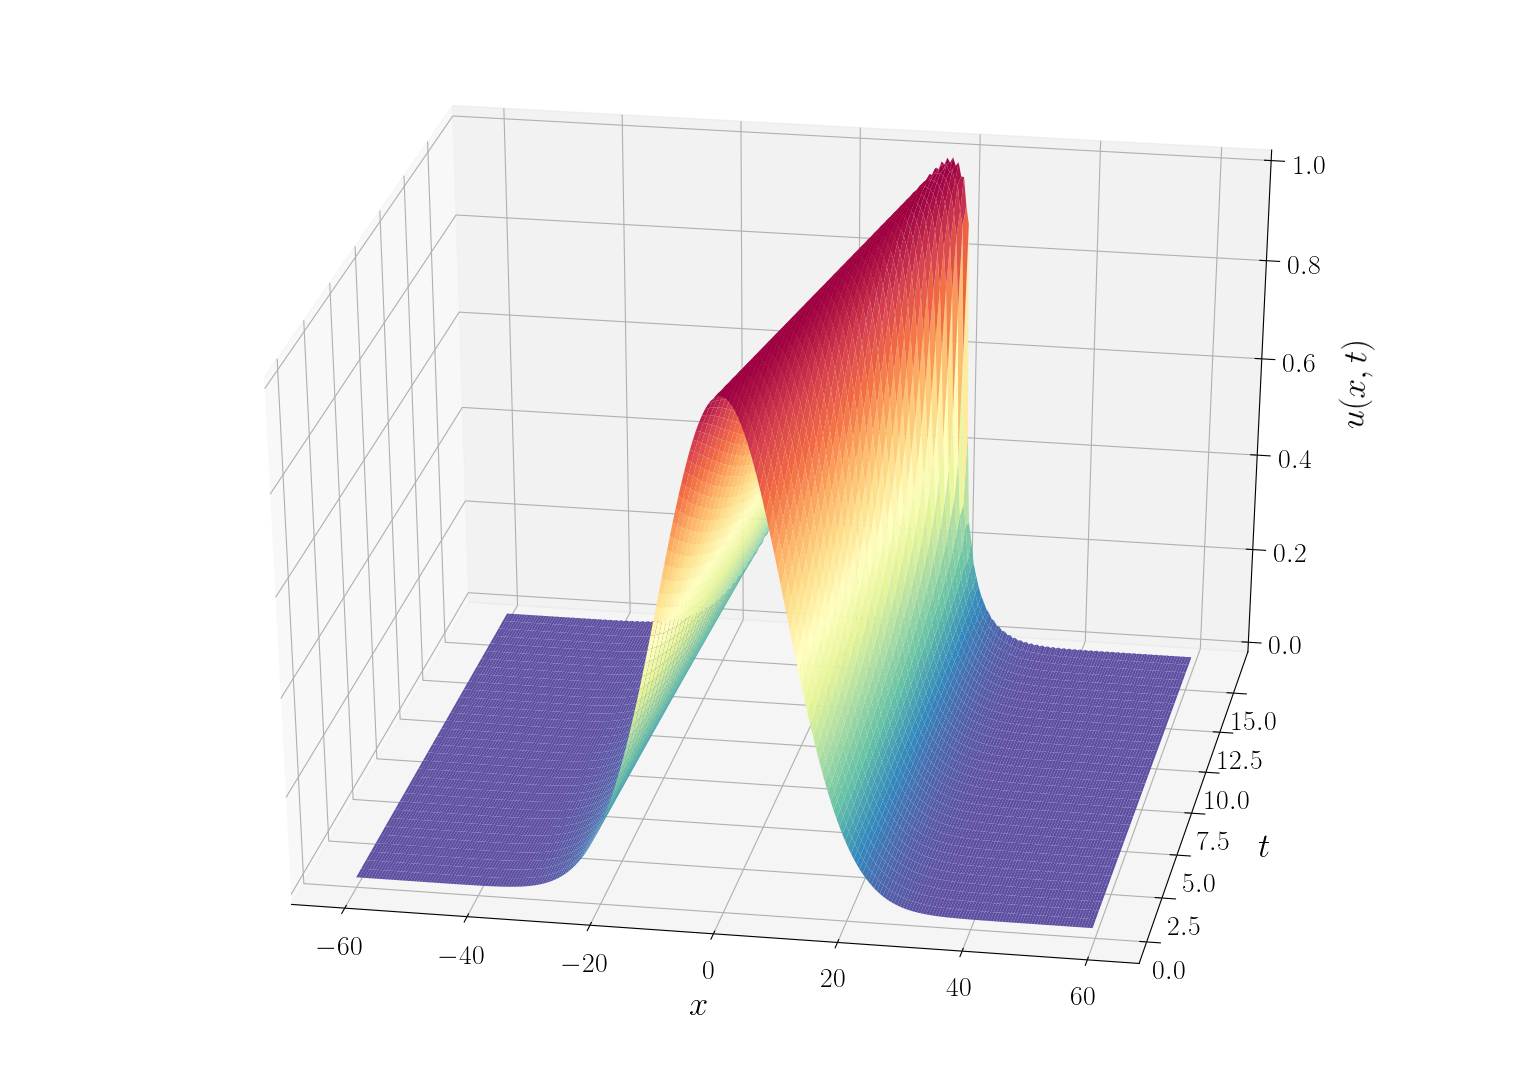
\includegraphics[width=12cm]{burgers_equation/deterministic/numerical_experiments/inviscid/figures/small_alpha.png}
		\caption{Numerical solution for (\ref{IVP_Burgers}) using (\ref{Galerkin_Euler}) with $\alpha = 1.0 \times 10^{-5}$, $N=256$, and $\Delta t = 1.0 \times 10^{-3}$.}
		\vspace{2mm}
		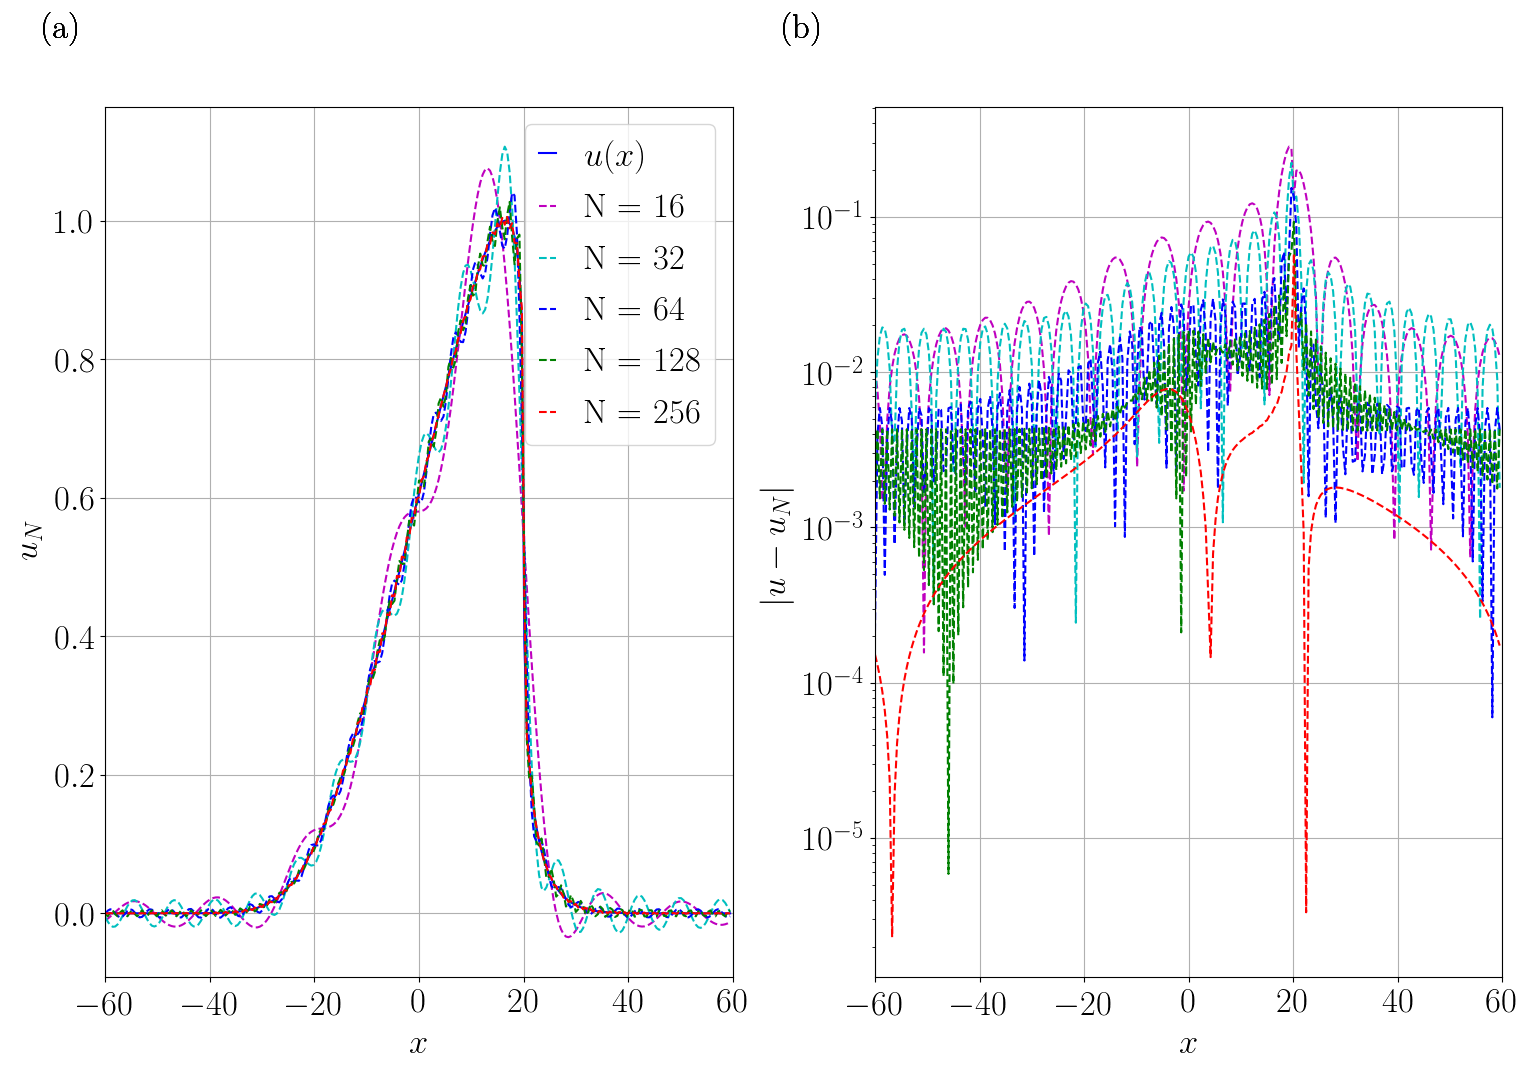
\includegraphics[width=12.5cm]{burgers_equation/deterministic/numerical_experiments/inviscid/figures/small_alpha_T.png}
		\caption{Numerical solution for (\ref{IVP_Burgers}) using (\ref{Galerkin_Euler}) at the time $T_c$ with $\alpha = 1.0 \times 10^{-5}$, and $\Delta t = 1.0 \times 10^{-3}$. (b) Point-wise error of approximation.}
	\end{figure}
	\newpage
	\begin{figure}[H]
		\centering	
		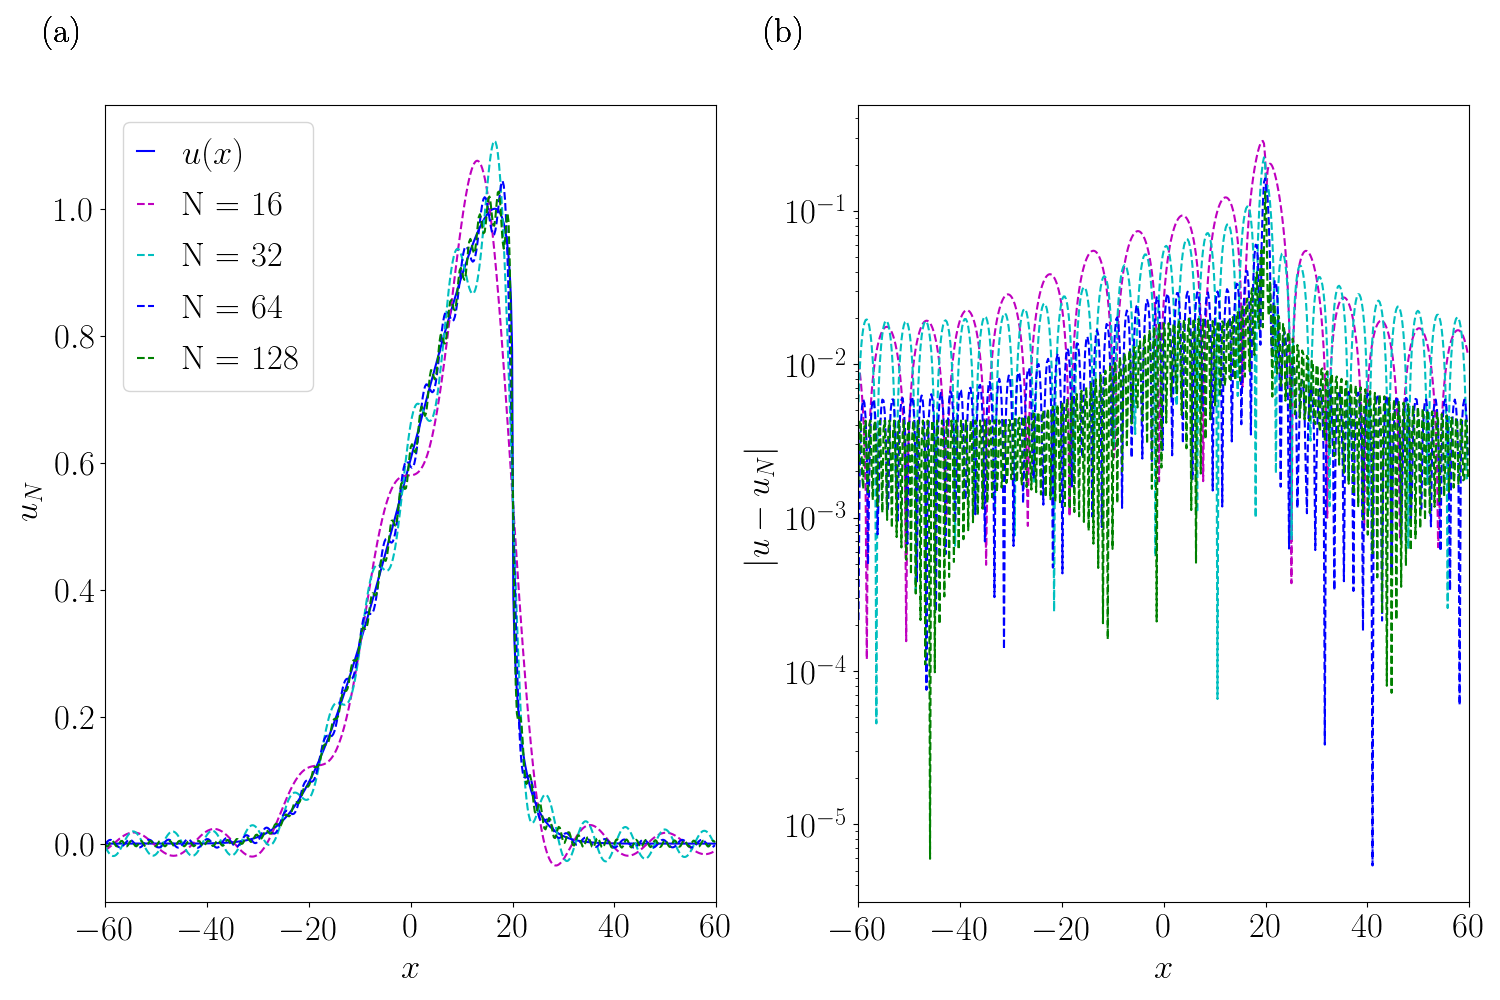
\includegraphics[width=13cm]{burgers_equation/deterministic/numerical_experiments/inviscid/figures/Numerical_Solution_Inviscid_T.png}
		\caption{(a) Exact solution for (\ref{IVP_Burgers}), and its approximations using (\ref{Galerkin_Euler}) at the time $Tc$ with initial condition $u_0(x) = e^{-0.005x^2}$, $x \in [-60, 60]$. (b) Pointwise error of approximation.}
		\label{convection_aprox_T}
		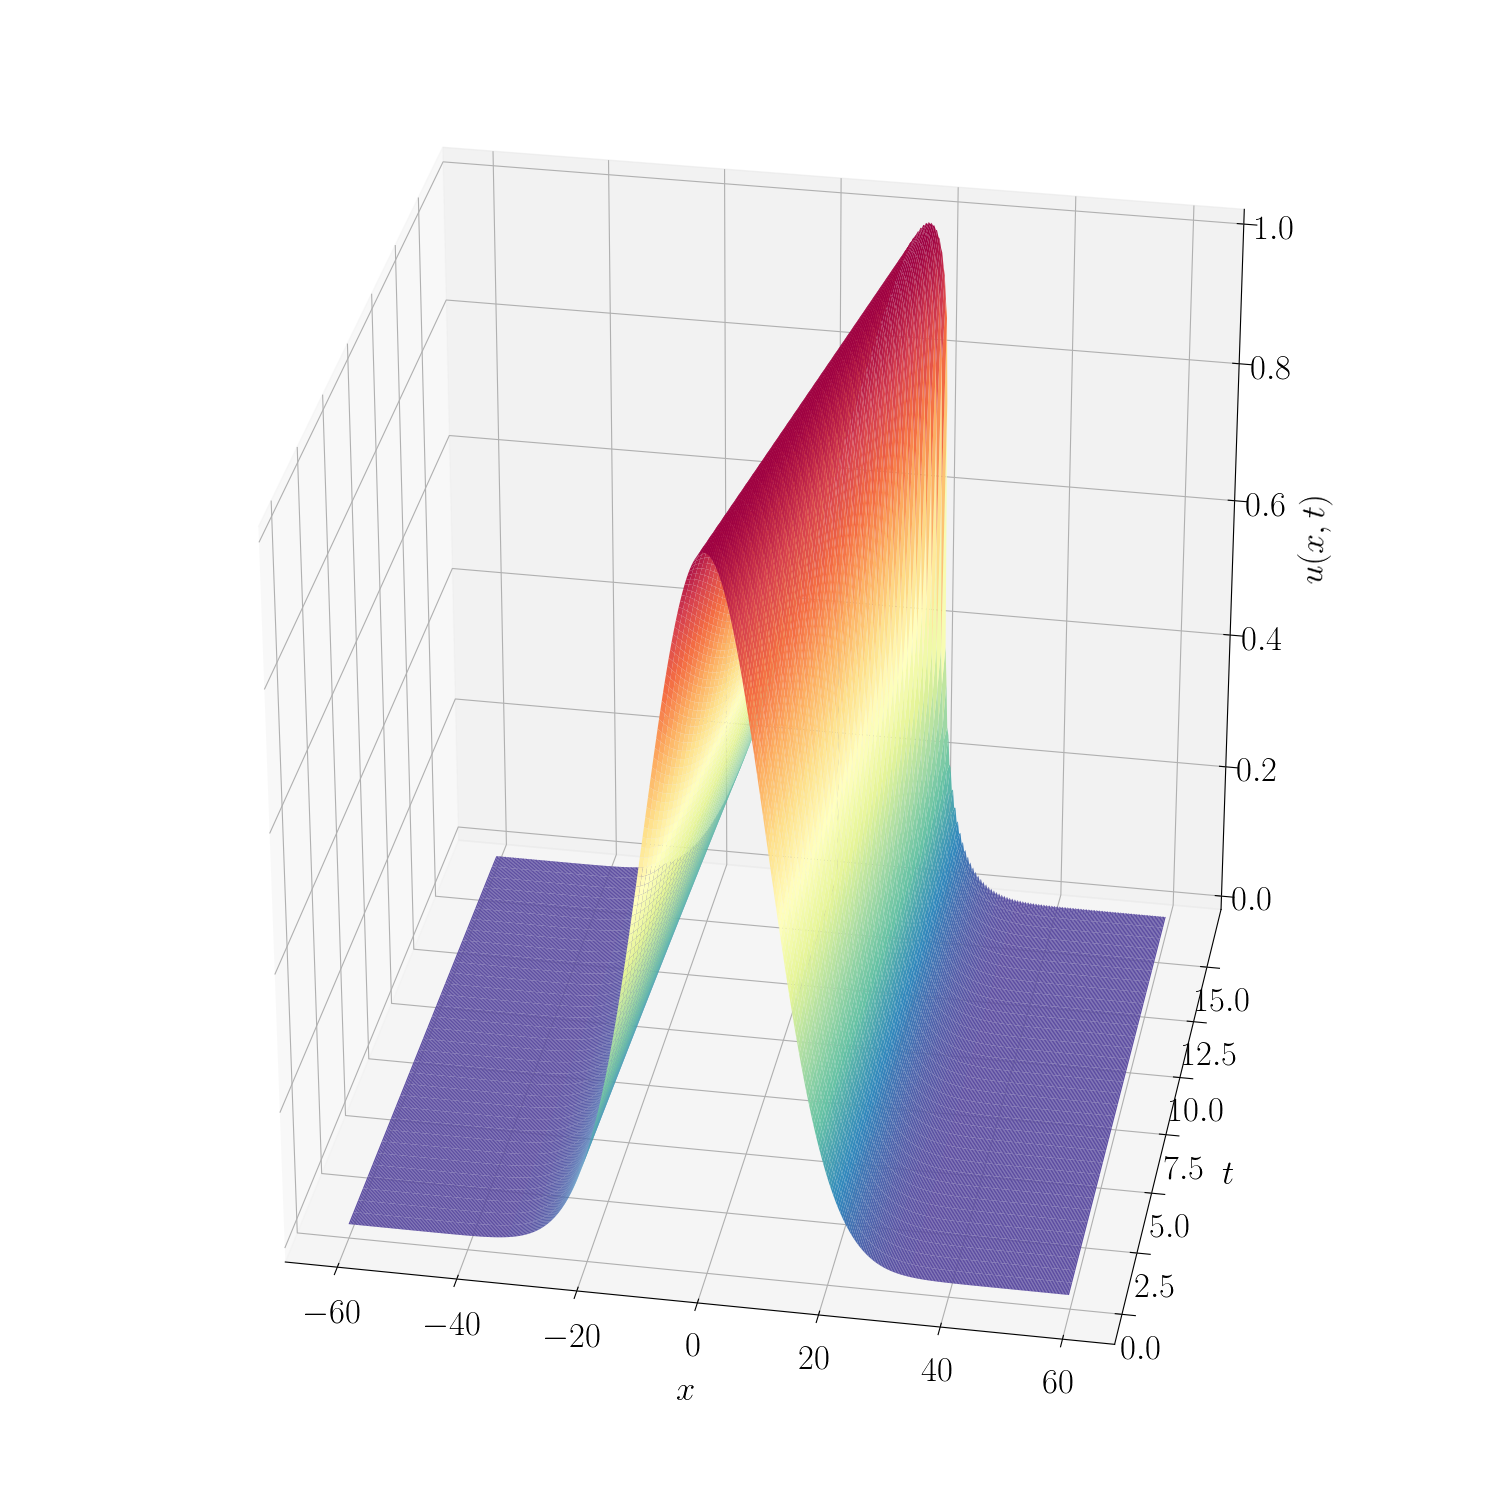
\includegraphics[width=11cm]{burgers_equation/deterministic/numerical_experiments/inviscid/figures/Numerical_Solution_Inviscid.png}
		\caption{Numerical approximation for  \ref{IVP_Burgers} using (\ref{Galerkin_Euler}) with $N=512$, $u_0(x) = e^{-0.005x^2}$, $x \in [-60, 60]$, and $t \in [0, Tc]$.}
	\end{figure}
	\newpage
	\begin{table}[H]
		\centering
		\begin{tabular}{lccc}
			\toprule
			\multicolumn{1}{c}{\hspace{6mm}\textbf{Expansion}} & \multicolumn{3}{c}{\textbf{Distance}} \\
			\hspace{12mm} $N$ & $\Delta t=1\times 10^{-2}$ & $\Delta t=1\times 10^{-3}$ & $\Delta t=1\times 10^{-4}$ \\
			\midrule
			\hspace{12mm} 16 & 0.285531 & 0.285732 & 0.285752 \\
			\midrule
			\hspace{12mm} 32 & 0.222737 & 0.223260 & 0.223312 \\
			\midrule
			\hspace{12mm} 64 & 0.160385 & 0.162782 & 0.163025 \\
			\midrule
			\hspace{12mm} 128 & 0.129297 & 0.133322 & 0.133733 \\
			\midrule
			\hspace{12mm} 256 & 0.083291 & 0.091449 & 0.092320 \\
			\bottomrule
		\end{tabular}
		\caption{Distance between exact solution for (\ref{IVP_Inviscid}) and the approximation for (\ref{IVP_Burgers}) with $\alpha = 1.0 \times 10^{-5}$.}
	\end{table}
	\begin{figure}[H]
		\centering
		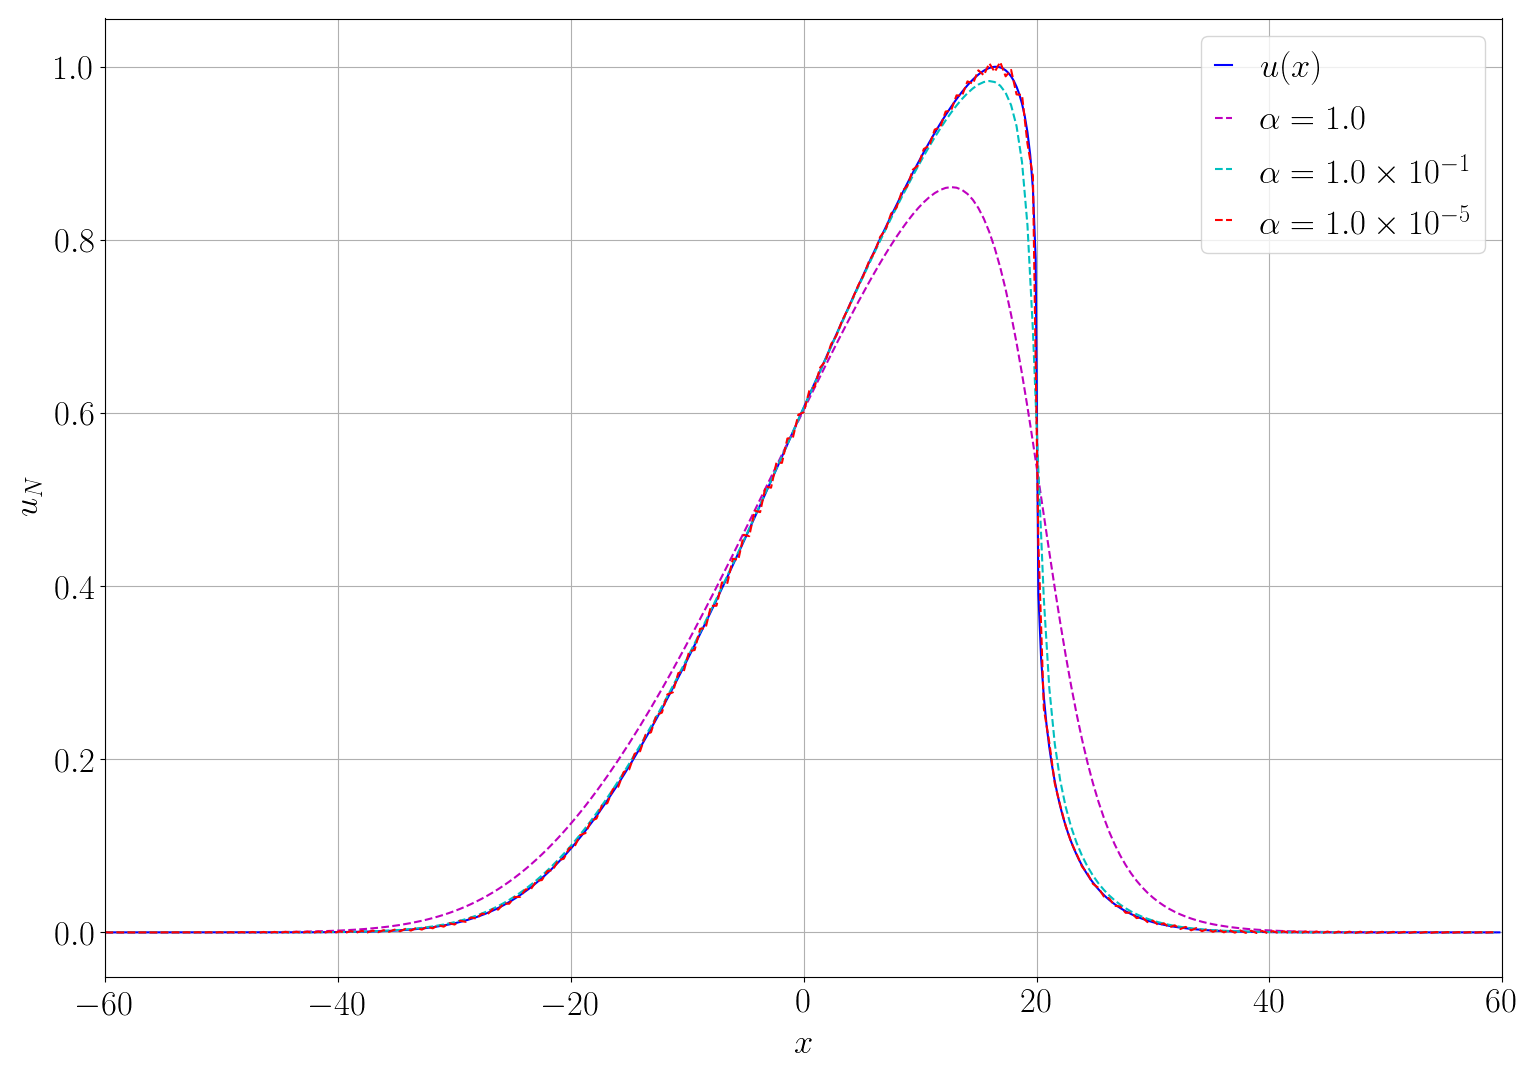
\includegraphics[width=12cm]{burgers_equation/deterministic/numerical_experiments/inviscid/figures/varios_alphas.png}
		\caption{Exact solution for (\ref{IVP_Inviscid}) and different approximations using (\ref{Galerkin_Euler}) with $N=256$, and $\Delta t = 1.0 \times 10^{-3}$.}
	\end{figure}